\chapter{Appendix}

%Test av tekstbokser under 
\newlist{todolist}{itemize}{2}
\setlist[todolist]{label=$\square$}

%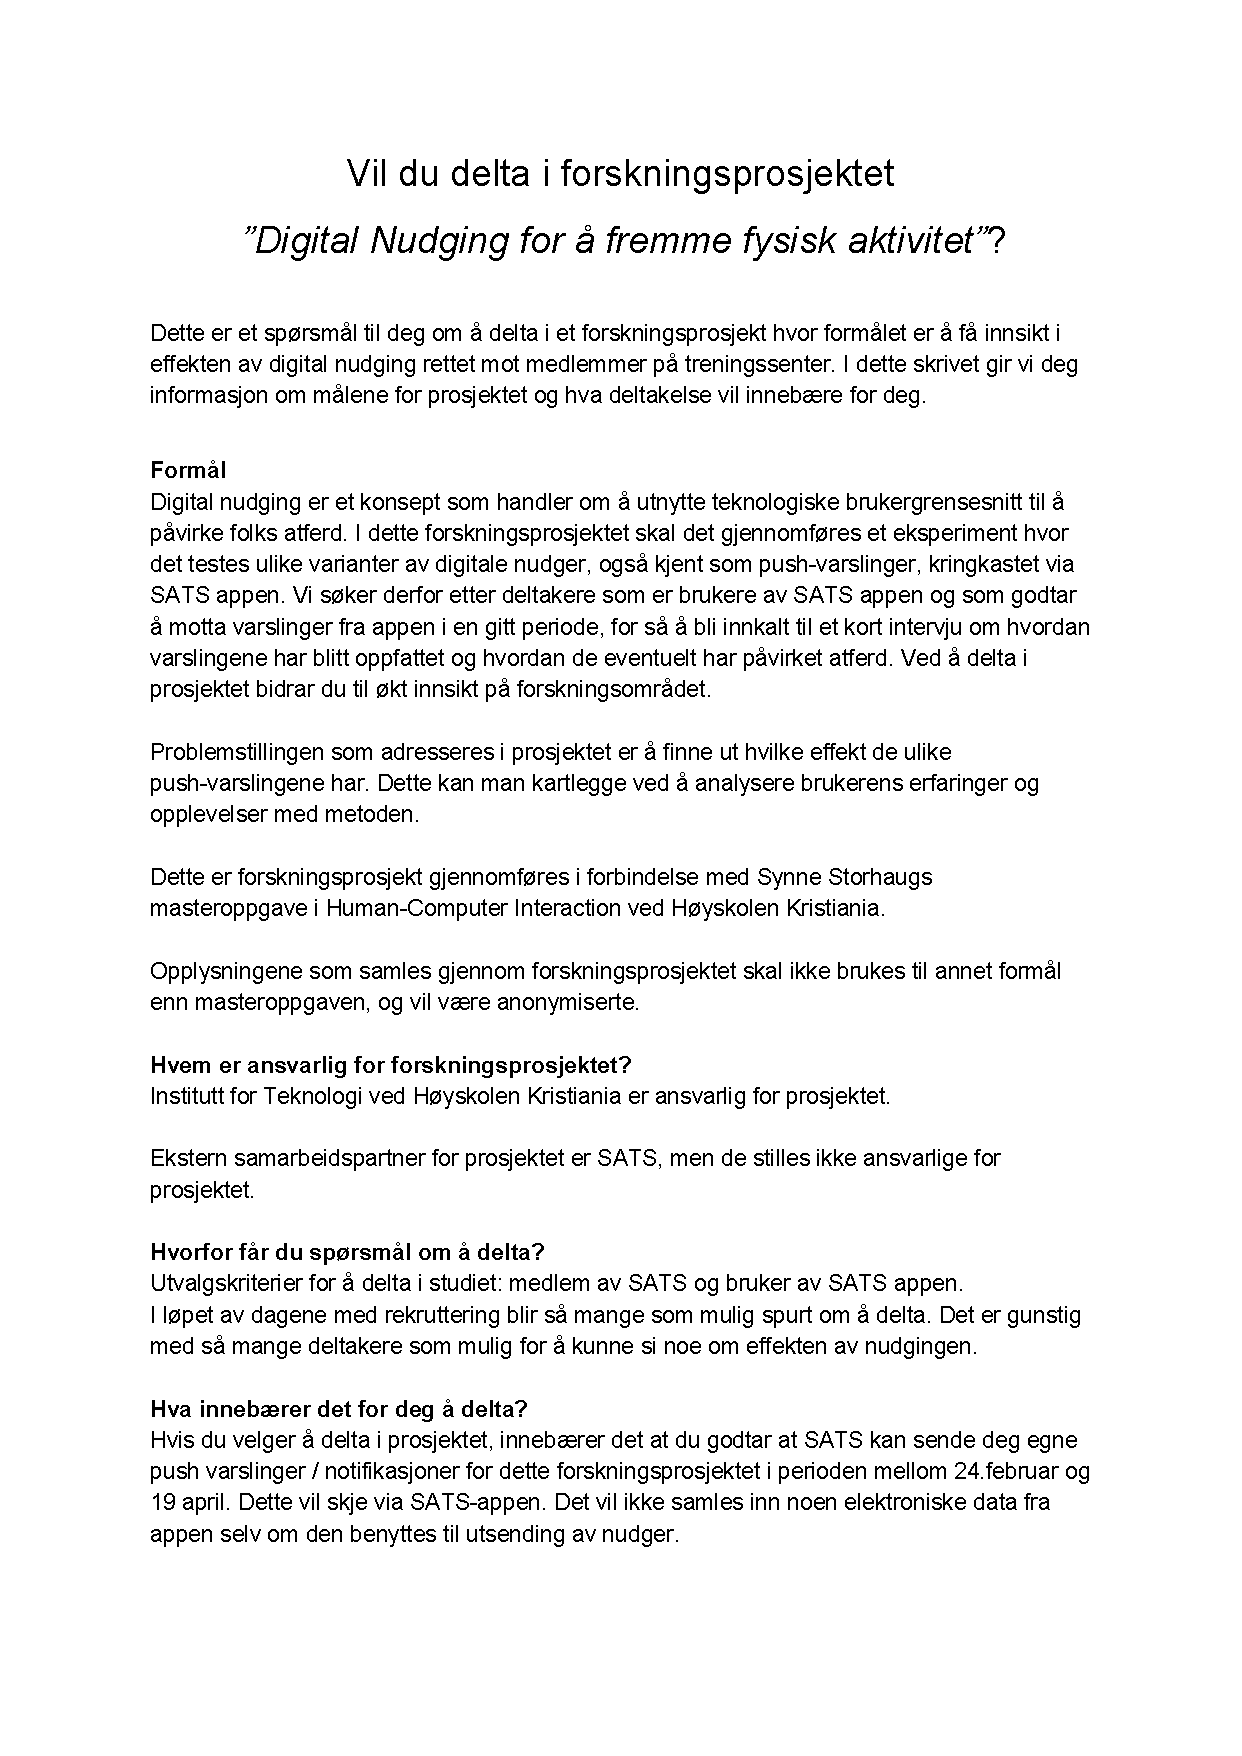
\includepdf[pages=-]{informasjon.pdf}

%Intervju guide
%Samtykkeskjema
%NSD 

\textbf{Vil du delta i forskningsprosjektet} \textbf{”Digital Nudging for å fremme fysisk aktivitet”?}
 \bigbreak
Dette er et spørsmål til deg om å delta i et forskningsprosjekt hvor formålet er å få innsikt i effekten av digital nudging rettet mot medlemmer på treningssenter. I dette skrivet gir vi deg informasjon om målene for prosjektet og hva deltakelse vil innebære for deg.
 
\textbf{Formål}
\bigbreak
Digital nudging er et konsept som handler om å utnytte teknologiske brukergrensesnitt til å påvirke folks atferd. I dette forskningsprosjektet skal det gjennomføres et eksperiment hvor det testes ulike varianter av digitale nudger, også kjent som push-varslinger, kringkastet via SATS appen. Vi søker derfor etter deltakere som er brukere av SATS appen og som godtar å motta varslinger fra appen i en gitt periode, for så å bli innkalt til et kort intervju om hvordan varslingene har blitt oppfattet og hvordan de eventuelt har påvirket atferd. Ved å delta i prosjektet bidrar du til økt innsikt på forskningsområdet. 
\bigbreak

Problemstillingen som adresseres i prosjektet er å finne ut hvilke effekt de ulike push-varslingene har. Dette kan man kartlegge ved å analysere brukerens erfaringer og opplevelser med metoden. 
\bigbreak

Dette er forskningsprosjekt gjennomføres i forbindelse med Synne Storhaugs masteroppgave i Human-Computer Interaction ved Høyskolen Kristiania.
\bigbreak
 
Opplysningene som samles gjennom forskningsprosjektet skal ikke brukes til annet formål enn masteroppgaven, og vil være anonymiserte. 
\bigbreak

\textbf{Hvem er ansvarlig for forskningsprosjektet?}
\bigbreak
Institutt for Teknologi ved Høyskolen Kristiania er ansvarlig for prosjektet.
Ekstern samarbeidspartner for prosjektet er SATS, men de stilles ikke ansvarlige for prosjektet.  
\textbf{Hvorfor får du spørsmål om å delta?}
\bigbreak
Utvalgskriterier for å delta i studiet: medlem av SATS og bruker av SATS appen. 
I løpet av dagene med rekruttering blir så mange som mulig spurt om å delta. Det er gunstig med så mange deltakere som mulig for å kunne si noe om effekten av nudgingen. 
 
\textbf{Hva innebærer det for deg å delta?}
\bigbreak
Hvis du velger å delta i prosjektet, innebærer det at du godtar at SATS kan sende deg egne push varslinger / notifikasjoner for dette forskningsprosjektet i perioden mellom 24.februar og 19 april. Dette vil skje via SATS-appen. Det vil ikke samles inn noen elektroniske data fra appen selv om den benyttes til utsending av nudger.

I tillegg innebærer det at du stiller opp på det intervju du vil bli tilkalt til en gang i løpet av mars måned. Om du ikke kan den gitte datoen, vil vi prøve å finne en dato det passer for deg. Intervjuet vil ta ca. 20 minutter. Intervjuet inneholder spørsmål om alder, kjønn, treningsvaner, treningsfrekvens, motivasjon, tanker, følelser, o.l. Dine svar blir registrert gjennom skriftlige notater. 

Vi kommer ikke til å samle inn opplysninger om deg fra andre kilder enn intervjuene.  
 
\textbf{Det er frivillig å delta}
\bigbreak
Det er frivillig å delta i prosjektet. Hvis du velger å delta, kan du når som helst trekke samtykke tilbake uten å oppgi noen grunn. Alle opplysninger om deg vil da bli anonymisert. Det vil ikke ha noen negative konsekvenser for deg hvis du ikke vil delta eller senere velger å trekke deg.
 
\textbf{Ditt personvern – hvordan vi oppbevarer og bruker dine opplysninger}
\bigbreak
Vi vil bare bruke opplysningene om deg til formålene vi har fortalt om i dette skrivet. Vi behandler opplysningene konfidensielt og i samsvar med personvernregelverket.
Det er bare prosjektansvarlig og student ved behandlingsansvarlig institusjon som vil ha tilgang på dine opplysninger.

For å sikre dine personopplysninger fra uvedkommende vil disse bli erstattet med en kode som lagres på egen navneliste adskilt fra øvrige data. Andre tiltak for å sikre oppbevaring og behandling av personopplysninger: flerfaktor autentisering, adgangsbegrensing, tastelås, innlåsing av dokumenter.  

Deltakere i prosjektet vil ikke kunne gjenkjennes ved publikasjonen. 

\textbf{Hva skjer med opplysningene dine når vi avslutter forskningsprosjektet?}
\bigbreak
Prosjektet skal etter planen avsluttes innen 22 juni 2020. Koblingsnøkkelen mellom deltaker og opplysninger slettes allerede etter arbeidet med intervjuet er ferdigstilt og dermed anonymiseres personopplysningene. De anonymiserte dataene vil beholdes utover prosjektperiodensslutt, og skal kun brukes ved eventuell videre forskning. Det er kun student og prosjektansvarlig som vil ha tilgang til disse. 
 
\textbf{Dine rettigheter}
\bigbreak
Så lenge du kan identifiseres i datamaterialet, har du rett til:

\begin{itemize}
\item innsyn i hvilke personopplysninger som er registrert om deg, 
\item å få rettet personopplysninger om deg,
\item få slettet personopplysninger om deg, 
\item få utlevert en kopi av dine personopplysninger (dataportabilitet)
\item å sende klage til personvernombudet eller Datatilsynet om behandlingen av dine personopplysninger.
\end{itemize}
 
\textbf{Hva gir oss rett til å behandle personopplysninger om deg?}
Vi behandler opplysninger om deg basert på ditt samtykke.
 
På oppdrag fra Institutt for Teknologi ved Høyskolen Kristiania har NSD – Norsk senter for forskningsdata AS vurdert at behandlingen av personopplysninger i dette prosjektet er i samsvar med personvernregelverket.
 
\textbf{Hvor kan jeg finne ut mer?}
Hvis du har spørsmål til studien, eller ønsker å benytte deg av dine rettigheter, ta kontakt med:
Institutt for Teknologi ved Høyskolen Kristiania på epost behandlingsansvarlig@kristiania.no 
Student Synne Storhaug på telefon 47387039 eller epost storsyn18@kristiania.no 
Prosjektansvarlig Siri Fagernes på telefon 41471542 eller epost siri.fagernes@kristiania.no 
Personvernombudet ved Høyskolen Kristiania på epost: personvernombud@kristiania.no  
NSD – Norsk senter for forskningsdata AS, på epost (personverntjenester@nsd.no) eller telefon: 55 58 21 17.
 
 
Med vennlig hilsen
 
Prosjektansvarlig                                       									Student
Siri Fagernes																					Synne Storhaug
 
 
-------------------------------------------------------------------------------------------------------------------------
\textbf{Samtykkeerklæring}
Jeg har mottatt og forstått informasjon om prosjektet “Digital Nudging for å fremme fysisk aktivitet”, og har fått anledning til å stille spørsmål. Jeg samtykker til:
 
 \begin{todolist}
    \item å delta i intervju i forbindelse med forskningen
    \item å motta push varslinger sendt ut i forbindelse med forskningsprosjektet i SATS appen i perioden mellom 24 februar til 19 april
       \item å sørge for at varslinger fra SATS appen er tillatt i innstillinger på telefonen i perioden for eksperimentet 
          \item at det blir lagret opplysninger om mine treningsvaner (helseopplysninger), gjort via intervju       
\end{todolist}

Jeg samtykker til at mine opplysninger behandles frem til prosjektet er avsluttet, ca. 22 juni 2020
 
 
---------------------------------------------------------------------------------------------------------------------------(Signert av prosjektdeltaker) 							(Dato)

